\documentclass[12pt,a4paper]{article}
\usepackage{ctex}
\usepackage{amsmath,amscd,amsbsy,amssymb,latexsym,url,bm,amsthm}
\usepackage{epsfig,graphicx,subfigure}
\usepackage{enumitem,balance}
\usepackage{wrapfig}
\usepackage{mathrsfs,euscript}
\usepackage[usenames]{xcolor}
\usepackage{hyperref}
\usepackage[vlined,ruled,linesnumbered]{algorithm2e}
\usepackage{array}
\hypersetup{colorlinks=true,linkcolor=black}

\newtheorem{theorem}{Theorem}
\newtheorem{lemma}[theorem]{Lemma}
\newtheorem{proposition}[theorem]{Proposition}
\newtheorem{corollary}[theorem]{Corollary}
\newtheorem{exercise}{Exercise}
\newtheorem*{solution}{Solution}
\newtheorem{definition}{Definition}
\theoremstyle{definition}

\renewcommand{\thefootnote}{\fnsymbol{footnote}}

\newcommand{\postscript}[2]
 {\setlength{\epsfxsize}{#2\hsize}
  \centerline{\epsfbox{#1}}}

\renewcommand{\baselinestretch}{1.0}

\setlength{\oddsidemargin}{-0.365in}
\setlength{\evensidemargin}{-0.365in}
\setlength{\topmargin}{-0.3in}
\setlength{\headheight}{0in}
\setlength{\headsep}{0in}
\setlength{\textheight}{10.1in}
\setlength{\textwidth}{7in}
\makeatletter \renewenvironment{proof}[1][Proof] {\par\pushQED{\qed}\normalfont\topsep6\p@\@plus6\p@\relax\trivlist\item[\hskip\labelsep\bfseries#1\@addpunct{.}]\ignorespaces}{\popQED\endtrivlist\@endpefalse} \makeatother
\makeatletter
\renewenvironment{solution}[1][Solution] {\par\pushQED{\qed}\normalfont\topsep6\p@\@plus6\p@\relax\trivlist\item[\hskip\labelsep\bfseries#1\@addpunct{.}]\ignorespaces}{\popQED\endtrivlist\@endpefalse} \makeatother

\begin{document}
\noindent

%========================================================================
\noindent\framebox[\linewidth]{\shortstack[c]{
\Large{\textbf{Lab07-Amortized Analysis}}\vspace{1mm}\\
CS214-Algorithm and Complexity, Xiaofeng Gao \& Lei Wang, Spring 2021.}}
\begin{center}
\footnotesize{\color{blue}$*$ Name:\underline{\quad   Haoyi You  \quad  }\quad Student ID:\underline{\quad 519030910193 \quad} \quad Email: \underline{\quad yuri-you@sjtu.edu.cn \quad}}
\end{center}
\begin{enumerate}
	\item Suppose we perform a sequence of n operations on a data structure in which the $i$ th 		operation costs $i$ if $i$ is an exact power of 2, and 1 otherwise. Use an accounting method to determine the amortized cost per operation.
	\begin{solution}
	Let $f(n)$ be the total cost of n operations.
	\begin{equation}
	    f(n)=\sum_{i=1}^{\lfloor logn \rfloor}2^i+(n-\lfloor logn \rfloor)
	\end{equation}
	So amortized cost per operation $g(n)$ is 
	\begin{equation}
	    g(n)=\frac{f(n)}{n}=\frac{2^{\lfloor logn \rfloor+1}-1+n-\lfloor logn \rfloor}{n} \le 3
	\end{equation}
	\end{solution}
	\item Consider an ordinary \textbf{binary min-heap} data structure with $n$ elements supporting
the instructions \textsc{Insert} and \textsc{Extract-Min} in $O(\log n)$ worst-case time. Give a
potential function $\Phi$ such that the amortized cost of \textsc{Insert} is $O(\log n)$ and the
amortized cost of \textsc{Extract-Min} is $O(1)$, and show that it works.
    
    \begin{solution}
        Assume $C_i$ is the cost of the $i^{th}$ operation, $\hat{C_i}=\Phi(S_i)-\Phi(S_{i-1})$.\\
        Let $\Phi(S_i)=n*log(n+1)$ with $n$ is the number of elements in binary min-heap.
        \begin{enumerate}
            \item $\forall n>0,n*log(n+1)-0*log0>0$.
            \item For \textsc{Insert} operation.
            \begin{equation}
            \begin{aligned}
                \hat{C_i}&=log(n)+n*log(n+1)-(n-1)log(n)\\&=n*log(n+1)-(n-2)*log(n)\\&
                =2log(n)+n*log(1+\frac{1}{n})\\&\le 2log(n)+n*(1+\frac{1}{n}-1)\\&
                =2log(n)+1
            \end{aligned}
            \end{equation}
            So the amortized cost of \textsc{Insert} is O(log(n)).
            \item For \textsc{Extract-Min} operation.
            \begin{equation}
            \begin{aligned}
                \hat{C_i}&=log(n)-(n-1)log(n)+(n-2)log(n-1)\\&
                \le (n-1)log(1+\frac{1}{n-1})\\&=1
            \end{aligned}
            \end{equation}
            So the amortized cost of \textsc{Extract-Min} is O(1).
            \item The amortized cost analysis is based on the fact that if we take \textsc{Extract-Min} at $n$ elements, we must have taken \textsc{Insert} at $n-1$ elements before.
        \end{enumerate}
    \end{solution}
	\item Assume we have a set of arrays $A_0, A_1, A_2,\cdots$, where the $i^{th}$ array $A_i$ has a length of $2^i$. Whenever an element is inserted into the arrays, we always intend to insert it into $A_0$. If $A_0$ is full then we pop the element in $A_0$ off and insert it with the new element into $A_{1}$. (Thus, if $A_{i}$ is already full, we recursively pop all its members off and insert them with the elements popped from $A_0,...,A_{i-1}$ and the new element into $A_{i+1}$ until we find an empty array to store the elements.) An illustrative example is shown in Figure \ref{Fig-MultiArray}. Inserting or popping an element take $O(1)$ time.

	\begin{figure}[!htbp]
	\centering
	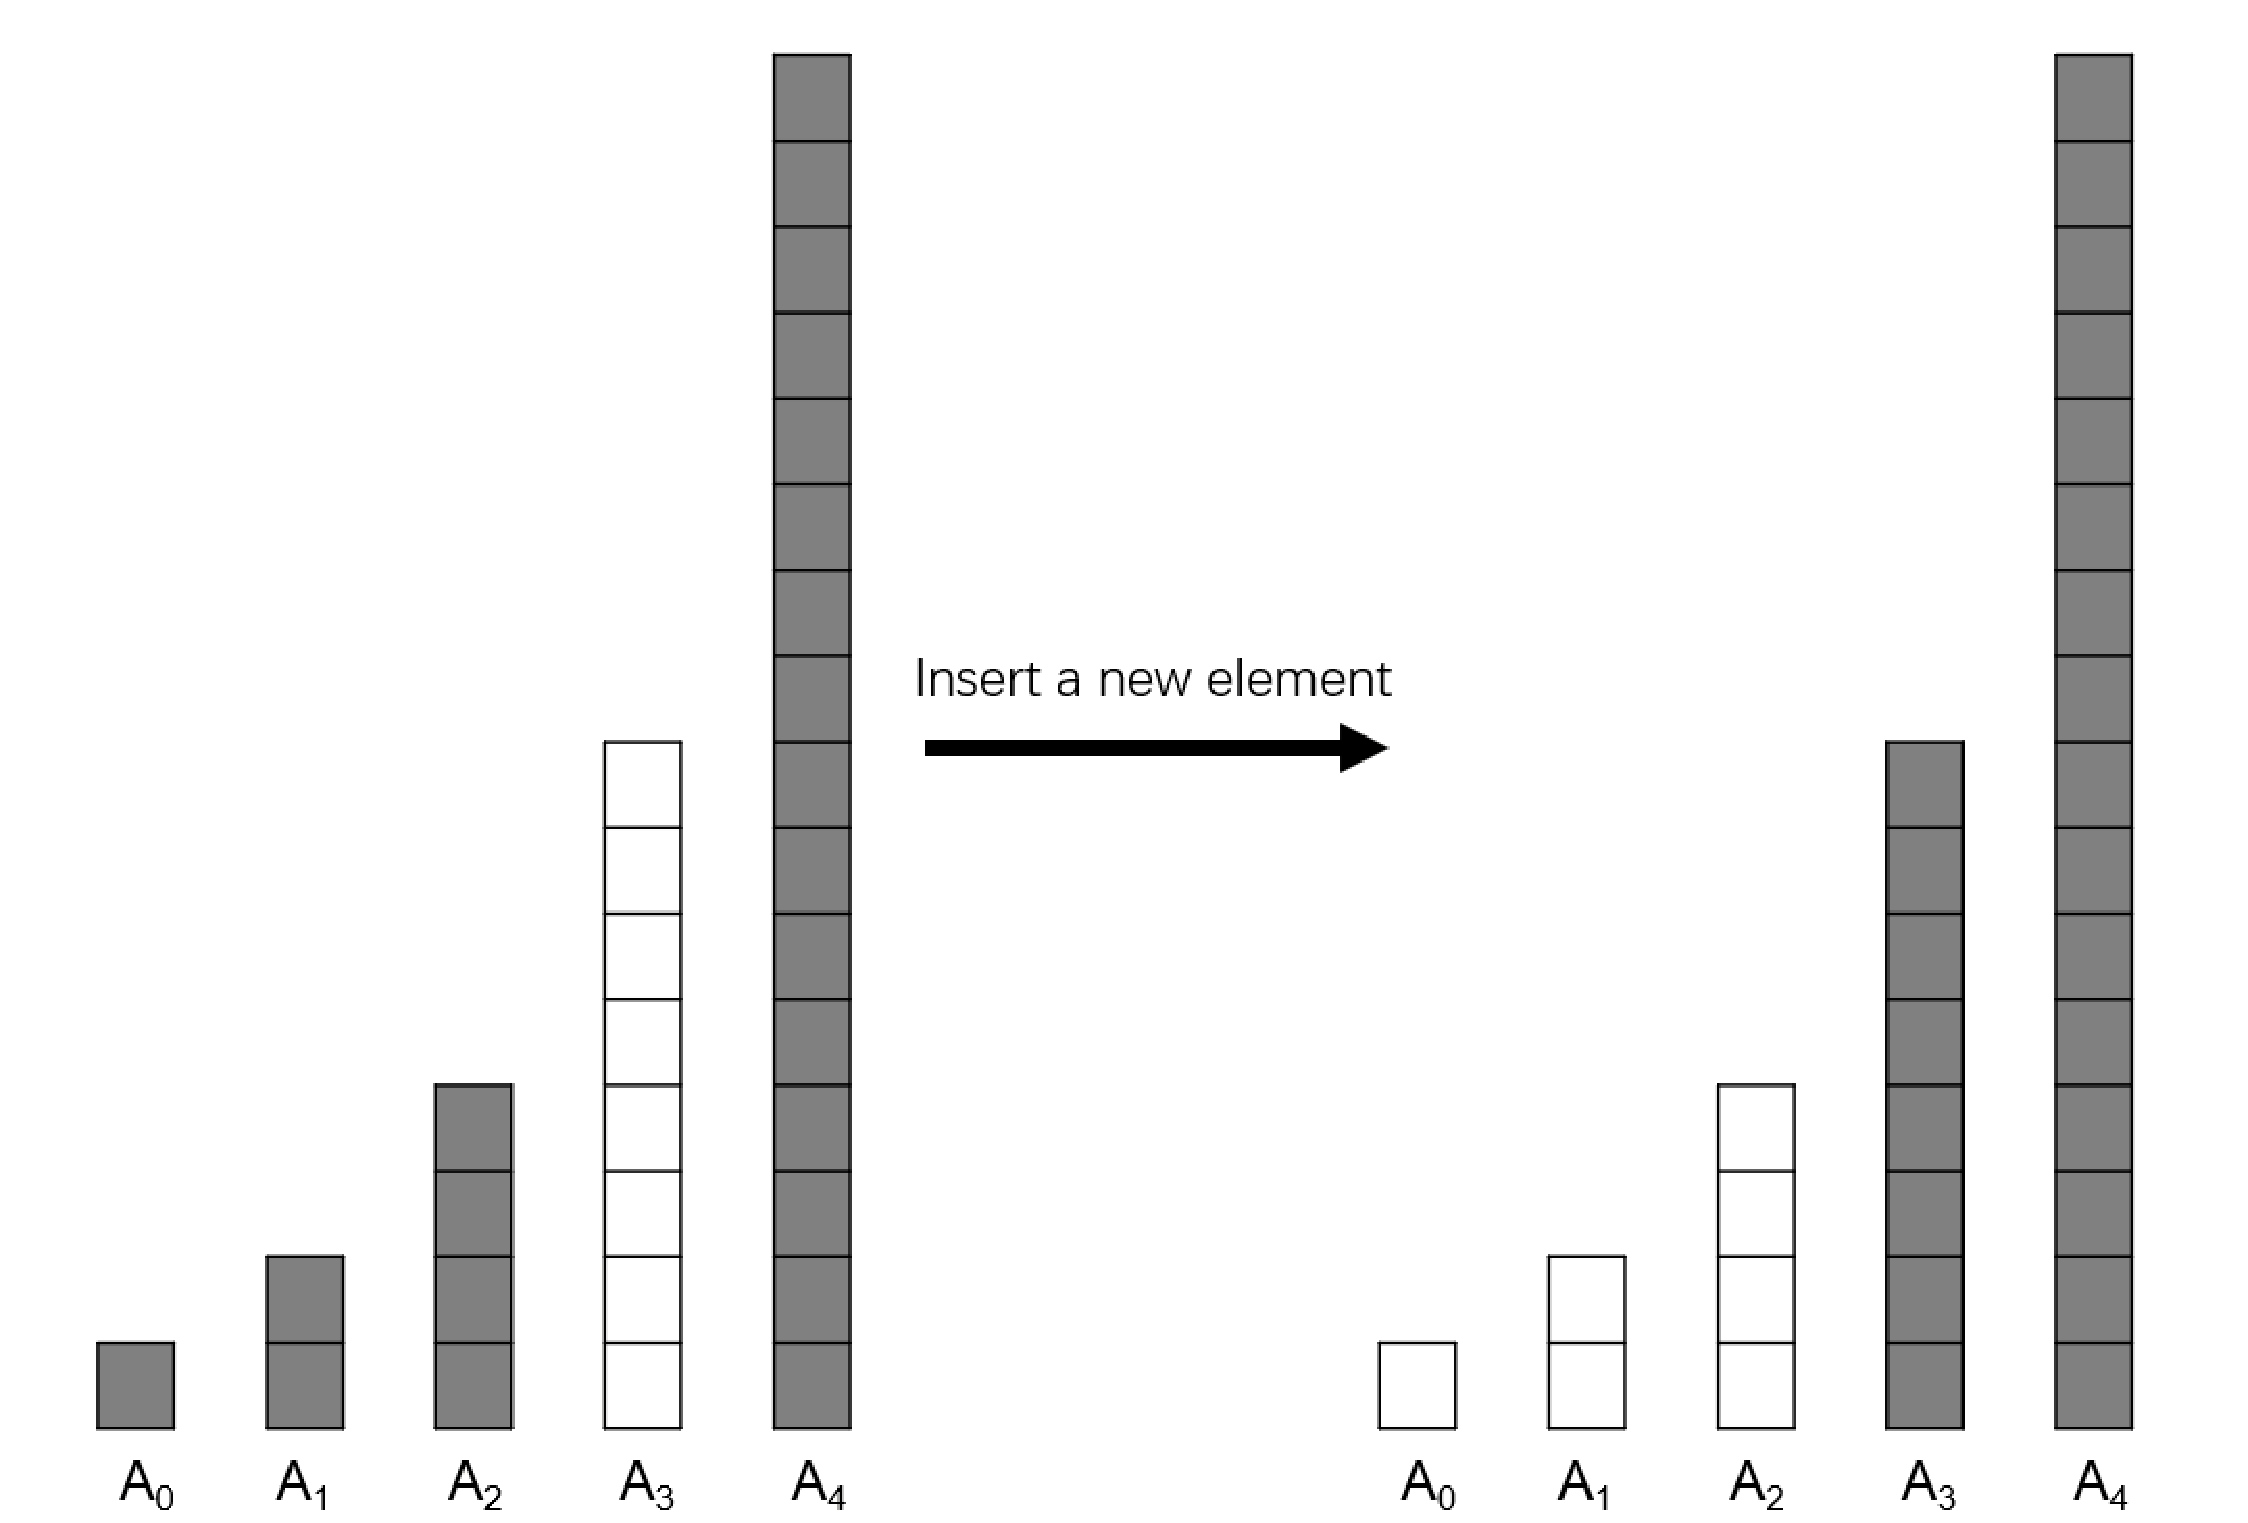
\includegraphics[width=0.5\textwidth]{Fig-MultiArray.pdf}
	\caption{An example of making room for one new element in the set of arrays.}
	\label{Fig-MultiArray}
	\end{figure}

    \begin{enumerate}
        \item In the worst case, how long does it take to add a new element into the set of arrays containing $n$ elements?
        \item Prove that the amortized cost of adding an element is $O(\log n)$ by \emph{Aggregation Analysis}.
        \item If each array $A_i$ is required to be sorted but elements in different arrays have no relationship with each other, how long does it take in the worst case to search an element in the arrays containing $n$ elements? 
\item What is the amortized cost of adding an element in the case of (c) if the comparison between two elements also takes $O(1)$ time?
    \end{enumerate}
	\begin{solution}
	\begin{enumerate}
	    \item If $n=2^i-1$,this time $A_0$~$A_{i-1}$ is full, it costs $\sum_{j=0}^{i-1}2^j+2^i=2n-1$ times.
	    \item
	    First we prove at any state, $\forall i,A_i$ is either empty or full. 
	    \begin{enumerate}
	        \item We assume there are $k$ elements in total.
	        \item When $k=1,A_0$ is full,others is empty.
	        \item Assume when $k=n-1$ the hypothesis is correct. 
	        \item This time we want to add a new element.Assume $j$ to be the minimum number that $A_i$ is empty at $k=n-1$. When we add the element,we find $A_0$\textasciitilde$A_{j-1}$ is full, we should pop them. And $A_0$\textasciitilde$A_{j-1}$ become empty. Here there are $2^j$ elements need inserting, so $A_j$ become full,which means when $k=n$,the hypothesis is still correct.
	        \item From the mathematical induction, $\forall n\in \mathbb{R}$, the hypothesis is correct.
	    \end{enumerate}
	    Then we know $\forall n\in \mathbb{R}$, we can write $n$ as $n=\sum_{i=0}^{n} b_i*2^i$. So $A_i$ is full iff $b_i=1$.\\
	    If we add from 0 to $n$, the $k^{th}$ bit of $n$ changes $\lfloor \frac{n}{2^k}\rfloor$ times. Every time changing means making $A_k$ from full to empty or from empty to full, which costs $2^k$ times.\\
	    So the amortized cost 
	    \begin{equation}
	        C_n=(\sum_{i=0}^{\lfloor log(n)\rfloor}2^i*\lfloor \frac{n}{2^i}\rfloor)/n=log(n)
	    \end{equation}
	    So the amortized cost is $O(log(n))$.
	    \item If the elements is in the last array or do not contained in the set of arrays.We must search from $A_0$\textasciitilde$A_{\lfloor log(n)\rfloor}$ and in each array we cost $log|A_i|=i$ times by binary search. So the total cost is 
	    \begin{equation}
	        \sum_{i=0}^{\lfloor log(n)\rfloor}i=\frac{(\lfloor log(n)\rfloor)(\lfloor log(n)\rfloor+1)}{2}\approx \frac{log^2n}{2}
	    \end{equation}
	    So the cost in worst case is $O(log^2n)$.
        \item Based on the proof in (b), add an elements means change $A_j$ from empty to full and change $A_0$\textasciitilde$A_{j-1}$ from full to empty. So we need to pop $A_0$\textasciitilde$A_{j-1}$ and insert them in $A_j$. The pop operation costs $\sum_{i=0}^{j-1}2^i=2^j-1$. The insert operation we use merge sort and costs $O(2^j)$. So the total cost is $O(2^j)$ with $j$ is changed from empty to full.\\
        So the total cost add from $0$ to $n$ is 
        \begin{equation}
            \sum_{i=0}^{\lfloor log(n)\rfloor}O(2^i)*\lfloor \frac{n}{2^i}\rfloor)=O(nlog(n)).
        \end{equation}
        So the amortized cost is $O(nlog(n))/n=O(log(n))$.
	\end{enumerate}
	\end{solution}
\end{enumerate}



\textbf{Remark:} Please include your .pdf, .tex files for uploading with standard file names.


%========================================================================
\end{document}
